\definecolor{failink}{HTML}{20252A}
\definecolor{failmuted}{HTML}{6B737A}
\definecolor{failblue}{HTML}{356FA8}
\definecolor{failorange}{HTML}{C47A36}
\definecolor{failred}{HTML}{B44747}
\definecolor{failpurple}{HTML}{7658A5}
\definecolor{failfill}{HTML}{F7F9FA}

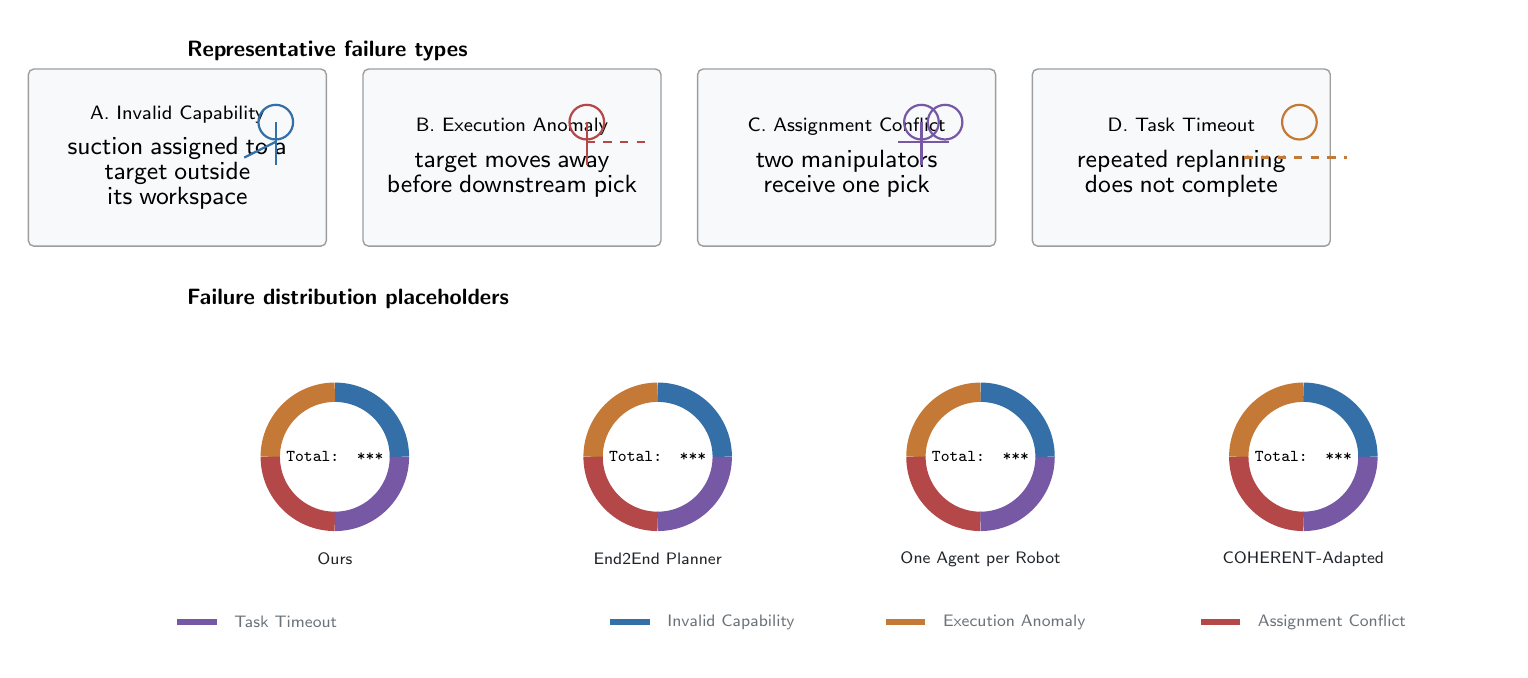
\begin{tikzpicture}[
  x=1cm,y=1cm,
  font=\sffamily\fontsize{6.8}{7.6}\selectfont,
  card/.style={draw=failink!45,fill=failfill,rounded corners=2pt,
               line width=.5pt,align=center},
  title/.style={font=\sffamily\bfseries\fontsize{7.6}{8.4}\selectfont},
  small/.style={font=\sffamily\fontsize{5.8}{6.5}\selectfont,text=failmuted},
  donut/.style={line width=7pt}
]
  \node[title,anchor=west] at (0,7.8) {Representative failure types};
  \foreach \x/\head/\body in {
    0/{A. Invalid Capability}/{suction assigned to a\\target outside its workspace},
    4.25/{B. Execution Anomaly}/{target moves away\\before downstream pick},
    8.50/{C. Assignment Conflict}/{two manipulators\\receive one pick},
    12.75/{D. Task Timeout}/{repeated replanning\\does not complete}}{
    \node[card,text width=3.55cm,minimum height=2.25cm] at (\x,6.45)
      {\head\\[2pt]\small \body};
  }
  % Minimal scene glyphs inside the four cards.
  \draw[failblue,line width=.8pt] (1.25,6.9) circle (.22);
  \draw[failblue,line width=.8pt] (1.25,6.9)--(1.25,6.35);
  \draw[failblue,line width=.8pt] (1.25,6.65)--(.85,6.45);
  \draw[failred,line width=.8pt] (5.2,6.9) circle (.22);
  \draw[failred,line width=.8pt] (5.2,6.9)--(5.2,6.35);
  \draw[failred,dashed,line width=.8pt] (5.2,6.65)--(6.0,6.65);
  \draw[failpurple,line width=.8pt] (9.45,6.9) circle (.22);
  \draw[failpurple,line width=.8pt] (9.45,6.9)--(9.45,6.35);
  \draw[failpurple,line width=.8pt] (9.15,6.65)--(9.8,6.65);
  \draw[failpurple,line width=.8pt] (9.75,6.9) circle (.22);
  \draw[failorange,line width=.8pt] (14.25,6.9) circle (.22);
  \draw[failorange,dashed,line width=.8pt] (13.55,6.45)--(14.85,6.45);
  \node[title,anchor=west] at (0,4.65) {Failure distribution placeholders};

  \foreach \x/\method in {2.0/Ours,6.1/End2End Planner,
                          10.2/One Agent per Robot,14.3/COHERENT-Adapted}{
    \draw[failblue,donut] (\x,2.65) ++(0:0.82) arc (0:90:0.82);
    \draw[failorange,donut] (\x,2.65) ++(90:0.82) arc (90:180:0.82);
    \draw[failred,donut] (\x,2.65) ++(180:0.82) arc (180:270:0.82);
    \draw[failpurple,donut] (\x,2.65) ++(270:0.82) arc (270:360:0.82);
    \node[font=\sffamily\bfseries\fontsize{6.5}{7.2}\selectfont] at (\x,2.65)
      {\texttt{Total: ***}};
    \node[small,text=failink] at (\x,1.35) {\method};
  }
  \draw[failblue,line width=2pt] (5.5,.55)--(6.0,.55);
  \node[small,anchor=west] at (6.1,.55) {Invalid Capability};
  \draw[failorange,line width=2pt] (9.0,.55)--(9.5,.55);
  \node[small,anchor=west] at (9.6,.55) {Execution Anomaly};
  \draw[failred,line width=2pt] (13.0,.55)--(13.5,.55);
  \node[small,anchor=west] at (13.6,.55) {Assignment Conflict};
  \draw[failpurple,line width=2pt] (0,.55)--(.5,.55);
  \node[small,anchor=west] at (.6,.55) {Task Timeout};
  \path[use as bounding box] (-.25,.2) rectangle (16.8,8.1);
\end{tikzpicture}
